
\documentclass{article}

\usepackage[left=1.8cm,right=1.8cm, top=2cm, bottom = 2cm]{geometry}
\usepackage{amsfonts}

\usepackage{amsmath}
\usepackage{xcolor}

\usepackage{tikz}
\usepackage{subfigure}

\usepackage{pgfplots}

\pgfplotsset{compat=1.10}
\usepgfplotslibrary{fillbetween}
\usetikzlibrary{patterns}



\pagestyle{empty}

\setlength{\tabcolsep}{15pt}


\newcommand{\deriv}[3][]{\frac{\mathrm{d}^{#1}#2}{\mathrm{d}#3^{#1}}}
\newcommand{\diff}{\;\mathrm{d}}

\newcommand{\norm}[1]{\left|\kern-1pt\left|#1\right|\kern-1pt\right|}
\newcommand{\bra}[1]{\left\langle #1 \,\right|}
\newcommand{\ket}[1]{\left|\, #1\right\rangle}
\newcommand{\braket}[2]{\left\langle #1 \mid #2 \right\rangle}




\begin{document}

\title{Convolutions}
\date{}

\maketitle
\thispagestyle{empty}

\Large

\vskip -10mm

\textbf{\underline{Objective: To understand the convolution of two functions and its}}

\textbf{\underline{relationship with multiplication.}}






\vspace{5mm}












\textbf{Warm-up: Cross-Correlation:}

\bigskip


Consider the functions $f(t)=\sin(t)$ and $g(t)=\cos(t)$. These functions are horizontal translations (phase shifts) of each other: $\sin(t)=\cos\left(t-\frac{\pi}{2}\right)$. Let's pretend we don't already know this; we will see how we could find the best amount to translate $\cos(t)$ by to make it similar to $\sin(t)$, using knowledge of the integrals of sine and cosine. This technique will then allow us to study more complicated functions than simple sinusoids.\medskip

The idea is that we will use the inner product of $\sin(t)$ and $\cos(t)$ on $L_2([0,2\pi])$ to compare how similar they are; but we will translate $\cos(t)$ by different amounts, to see how much we need to translate by to make the two functions as similar as possible.

The \textbf{cross-correlation} of $\sin(t)$ and $\cos(t)$ between $0$ and $2\pi$ is
\[\braket{\sin(\tau)}{\cos(\tau+t)}=\int_{0}^{2\pi}\sin(\tau)\cos(\tau+t)\diff \tau.\]

Note that previously we have used an inner product with a factor of $\frac{2}{L}$ in front; this isn't important, so for our current purposes we'll drop this factor, so technically this is a different inner product to the one we've used before, but it differs only by a constant factor, so it's essentially the same. This cross-correlation tells us, for a given $t$, how similar the sine and cosine waves are once the cosine is translated by $t$. See graphs overleaf.\bigskip


\begin{enumerate}
	\item Show that the cross-correlation of sine and cosine is given by
		\[\braket{\sin(\tau)}{\cos(\tau+t)}=-\pi\sin(t).\]
	\item Hence show that the maximum cross-correlation between sine and cosine occurs at $t=-\frac{\pi}{2}$; so $\cos\left(t-\frac{\pi}{2}\right)$ is the most similar a cosine wave can get to a sine wave. In this case, of course, $\cos\left(t-\frac{\pi}{2}\right)$ is actually equal to $\sin(t)$, but we can generalise this to pairs of functions where a simple translation does not turn one exactly into the other.
\end{enumerate}




\clearpage


\begin{center}
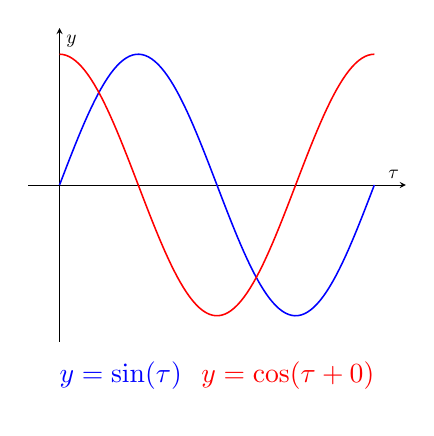
\begin{tikzpicture}[scale=0.7]
	\begin{axis}[axis lines=middle,
		            xlabel=$\tau$,
		            ylabel=$y$,
	           	 enlargelimits,
           		 ytick=\empty,
		            xtick=\empty
           	 ]
		
		\addplot[name path=F,blue,thick,domain={0:6.28},samples=100] {2*sin(x*180/3.14)};

		\addplot[name path=G,red,thick,domain={0:6.28},samples=100] {2*cos((x+0*0.785)*180/3.14)};
	\end{axis}
		\matrix[below] at (current bounding box.south){
			\node[blue,left] {$y=\sin(\tau)$};
			\node[red,right] {$y=\cos(\tau+0)$};\\
		};
\end{tikzpicture}
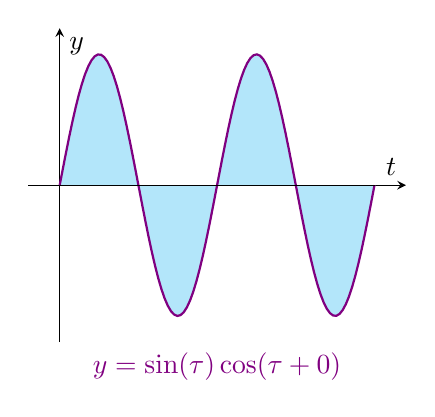
\begin{tikzpicture}[scale=0.7]
	\begin{axis}[axis lines=middle,
		            xlabel=$t$,
		            ylabel=$y$,
	           	 enlargelimits,
           		 ytick=\empty,
		            xtick=\empty
           	 ]
		
		\addplot[name path=F,violet,thick,domain={0:6.28},samples=100] {2*sin(x*180/3.14)*cos((x+0*0.785)*180/3.14)};

		\addplot[name path=G,domain=0:6.28] {0};

		\addplot[cyan!30] fill between [of=F and G];
	\end{axis}
	\node[below,violet] at (current bounding box.south) {$y=\sin(\tau)\cos(\tau+0)$};
\end{tikzpicture}
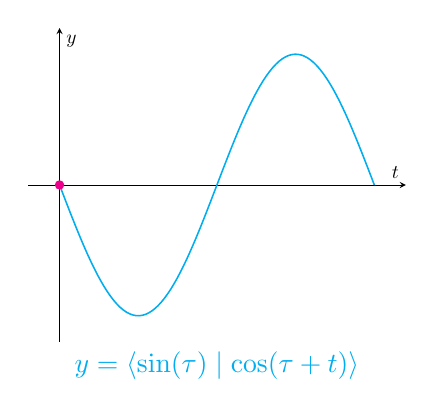
\begin{tikzpicture}[scale=0.7]
	\begin{axis}[axis lines=middle,
		            xlabel=$t$,
		            ylabel=$y$,
	           	 enlargelimits,
           		 ytick=\empty,
		            xtick=\empty
           	 ]
		
		\addplot[name path=F,cyan,thick,domain={0:6.28},samples=100] {-3.14*sin(x*180/3.14)};
		\addplot[magenta,thick,mark=*] coordinates{({0*0.785},{-3.14*sin((0*0.785)*180/3.14))})};
	\end{axis}
	\node[below,cyan] at (current bounding box.south) {$y=\braket{\sin(\tau)}{\cos(\tau+t)}$};
\end{tikzpicture}




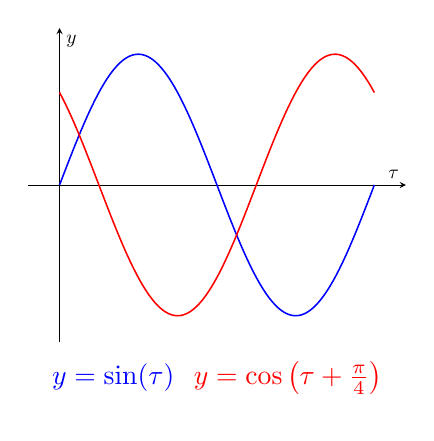
\begin{tikzpicture}[scale=0.7]
	\begin{axis}[axis lines=middle,
		            xlabel=$\tau$,
		            ylabel=$y$,
	           	 enlargelimits,
           		 ytick=\empty,
		            xtick=\empty
           	 ]
		
		\addplot[name path=F,blue,thick,domain={0:6.28},samples=100] {2*sin(x*180/3.14)};

		\addplot[name path=G,red,thick,domain={0:6.28},samples=100] {2*cos((x+1*0.785)*180/3.14)};
	\end{axis}
		\matrix[below] at (current bounding box.south){
			\node[blue,left] {$y=\sin(\tau)$};
			\node[red,right] {$y=\cos\left(\tau+\frac{\pi}{4}\right)$};\\
		};
\end{tikzpicture}
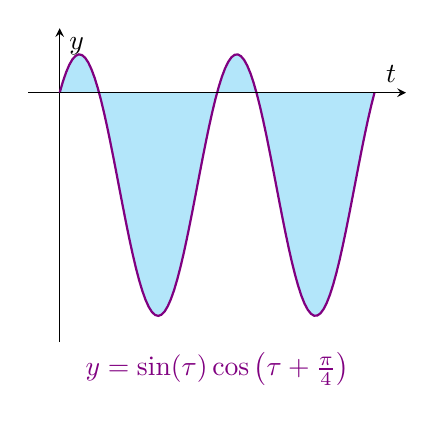
\begin{tikzpicture}[scale=0.7]
	\begin{axis}[axis lines=middle,
		            xlabel=$t$,
		            ylabel=$y$,
	           	 enlargelimits,
           		 ytick=\empty,
		            xtick=\empty
           	 ]
		
		\addplot[name path=F,violet,thick,domain={0:6.28},samples=100] {2*sin(x*180/3.14)*cos((x+1*0.785)*180/3.14)};

		\addplot[name path=G,domain=0:6.28] {0};

		\addplot[cyan!30] fill between [of=F and G];
	\end{axis}
	\node[below,violet] at (current bounding box.south) {$y=\sin(\tau)\cos\left(\tau+\frac{\pi}{4}\right)$};
\end{tikzpicture}
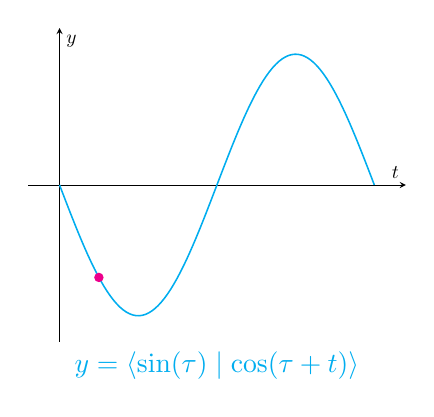
\begin{tikzpicture}[scale=0.7]
	\begin{axis}[axis lines=middle,
		            xlabel=$t$,
		            ylabel=$y$,
	           	 enlargelimits,
           		 ytick=\empty,
		            xtick=\empty
           	 ]
		
		\addplot[name path=F,cyan,thick,domain={0:6.28},samples=100] {-3.14*sin(x*180/3.14)};
		\addplot[magenta,thick,mark=*] coordinates{({1*0.785},{-3.14*sin((1*0.785)*180/3.14))})};
	\end{axis}
	\node[below,cyan] at (current bounding box.south) {$y=\braket{\sin(\tau)}{\cos(\tau+t)}$};
\end{tikzpicture}




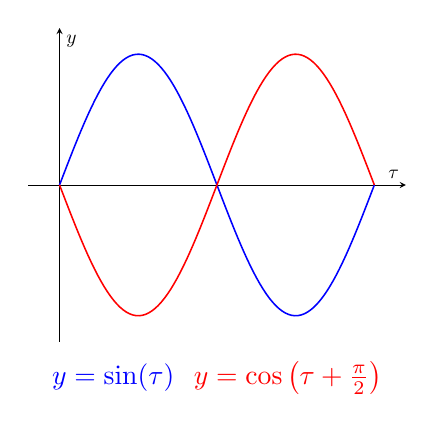
\begin{tikzpicture}[scale=0.7]
	\begin{axis}[axis lines=middle,
		            xlabel=$\tau$,
		            ylabel=$y$,
	           	 enlargelimits,
           		 ytick=\empty,
		            xtick=\empty
           	 ]
		
		\addplot[name path=F,blue,thick,domain={0:6.28},samples=100] {2*sin(x*180/3.14)};

		\addplot[name path=G,red,thick,domain={0:6.28},samples=100] {2*cos((x+2*0.785)*180/3.14)};
	\end{axis}
		\matrix[below] at (current bounding box.south){
			\node[blue,left] {$y=\sin(\tau)$};
			\node[red,right] {$y=\cos\left(\tau+\frac{\pi}{2}\right)$};\\
		};
\end{tikzpicture}
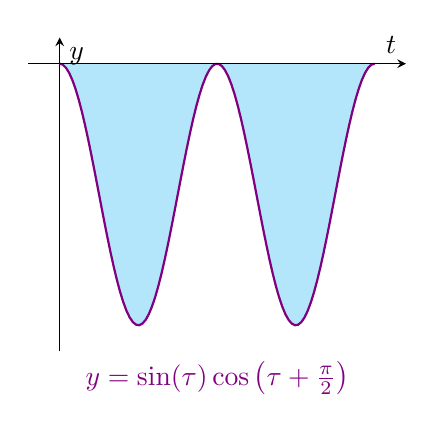
\begin{tikzpicture}[scale=0.7]
	\begin{axis}[axis lines=middle,
		            xlabel=$t$,
		            ylabel=$y$,
	           	 enlargelimits,
           		 ytick=\empty,
		            xtick=\empty
           	 ]
		
		\addplot[name path=F,violet,thick,domain={0:6.28},samples=100] {2*sin(x*180/3.14)*cos((x+2*0.785)*180/3.14)};

		\addplot[name path=G,domain=0:6.28] {0};

		\addplot[cyan!30] fill between [of=F and G];
	\end{axis}
	\node[below,violet] at (current bounding box.south) {$y=\sin(\tau)\cos\left(\tau+\frac{\pi}{2}\right)$};
\end{tikzpicture}
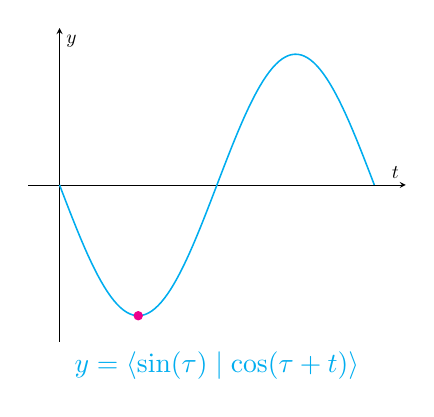
\begin{tikzpicture}[scale=0.7]
	\begin{axis}[axis lines=middle,
		            xlabel=$t$,
		            ylabel=$y$,
	           	 enlargelimits,
           		 ytick=\empty,
		            xtick=\empty
           	 ]
		
		\addplot[name path=F,cyan,thick,domain={0:6.28},samples=100] {-3.14*sin(x*180/3.14)};
		\addplot[magenta,thick,mark=*] coordinates{({2*0.785},{-3.14*sin((2*0.785)*180/3.14))})};
	\end{axis}
	\node[below,cyan] at (current bounding box.south) {$y=\braket{\sin(\tau)}{\cos(\tau+t)}$};
\end{tikzpicture}




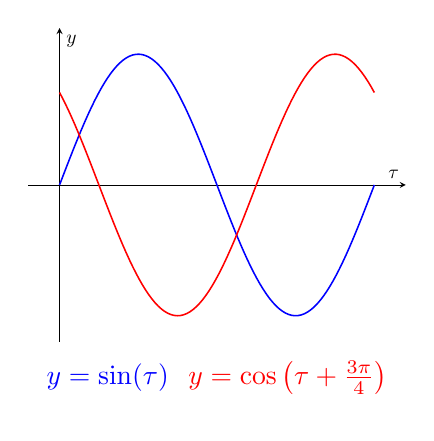
\begin{tikzpicture}[scale=0.7]
	\begin{axis}[axis lines=middle,
		            xlabel=$\tau$,
		            ylabel=$y$,
	           	 enlargelimits,
           		 ytick=\empty,
		            xtick=\empty
           	 ]
		
		\addplot[name path=F,blue,thick,domain={0:6.28},samples=100] {3*sin(x*180/3.14)};

		\addplot[name path=G,red,thick,domain={0:6.28},samples=100] {3*cos((x+1*0.785)*180/3.14)};
	\end{axis}
		\matrix[below] at (current bounding box.south){
			\node[blue,left] {$y=\sin(\tau)$};
			\node[red,right] {$y=\cos\left(\tau+\frac{3\pi}{4}\right)$};\\
		};
\end{tikzpicture}
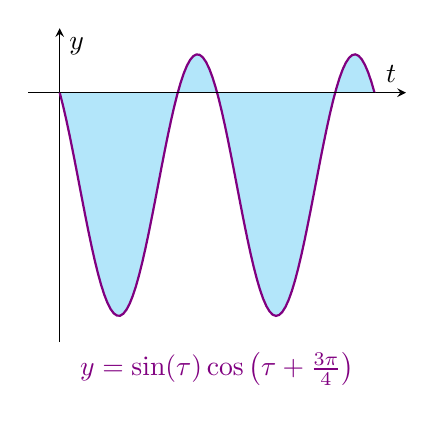
\begin{tikzpicture}[scale=0.7]
	\begin{axis}[axis lines=middle,
		            xlabel=$t$,
		            ylabel=$y$,
	           	 enlargelimits,
           		 ytick=\empty,
		            xtick=\empty
           	 ]
		
		\addplot[name path=F,violet,thick,domain={0:6.28},samples=100] {2*sin(x*180/3.14)*cos((x+3*0.785)*180/3.14)};

		\addplot[name path=G,domain=0:6.28] {0};

		\addplot[cyan!30] fill between [of=F and G];
	\end{axis}
	\node[below,violet] at (current bounding box.south) {$y=\sin(\tau)\cos\left(\tau+\frac{3\pi}{4}\right)$};
\end{tikzpicture}
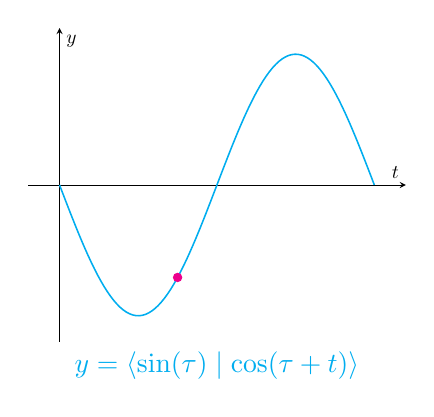
\begin{tikzpicture}[scale=0.7]
	\begin{axis}[axis lines=middle,
		            xlabel=$t$,
		            ylabel=$y$,
	           	 enlargelimits,
           		 ytick=\empty,
		            xtick=\empty
           	 ]
		
		\addplot[name path=F,cyan,thick,domain={0:6.28},samples=100] {-3.14*sin(x*180/3.14)};
		\addplot[magenta,thick,mark=*] coordinates{({3*0.785},{-3.14*sin((3*0.785)*180/3.14))})};
	\end{axis}
	\node[below,cyan] at (current bounding box.south) {$y=\braket{\sin(\tau)}{\cos(\tau+t)}$};
\end{tikzpicture}




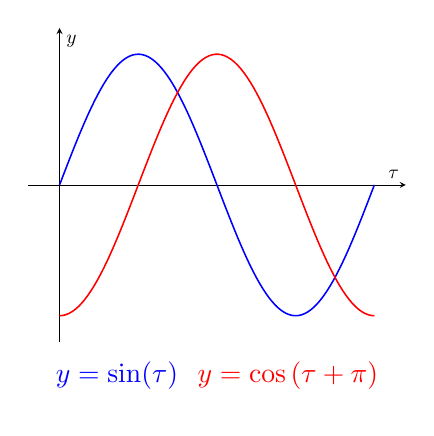
\begin{tikzpicture}[scale=0.7]
	\begin{axis}[axis lines=middle,
		            xlabel=$\tau$,
		            ylabel=$y$,
	           	 enlargelimits,
           		 ytick=\empty,
		            xtick=\empty
           	 ]
		
		\addplot[name path=F,blue,thick,domain={0:6.28},samples=100] {2*sin(x*180/3.14)};

		\addplot[name path=G,red,thick,domain={0:6.28},samples=100] {2*cos((x+4*0.785)*180/3.14)};
	\end{axis}
		\matrix[below] at (current bounding box.south){
			\node[blue,left] {$y=\sin(\tau)$};
			\node[red,right] {$y=\cos\left(\tau+\pi\right)$};\\
		};
\end{tikzpicture}
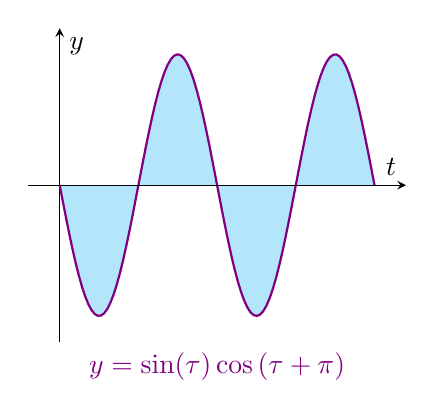
\begin{tikzpicture}[scale=0.7]
	\begin{axis}[axis lines=middle,
		            xlabel=$t$,
		            ylabel=$y$,
	           	 enlargelimits,
           		 ytick=\empty,
		            xtick=\empty
           	 ]
		
		\addplot[name path=F,violet,thick,domain={0:6.28},samples=100] {2*sin(x*180/3.14)*cos((x+4*0.785)*180/3.14)};

		\addplot[name path=G,domain=0:6.28] {0};

		\addplot[cyan!30] fill between [of=F and G];
	\end{axis}
	\node[below,violet] at (current bounding box.south) {$y=\sin(\tau)\cos\left(\tau+\pi\right)$};
\end{tikzpicture}
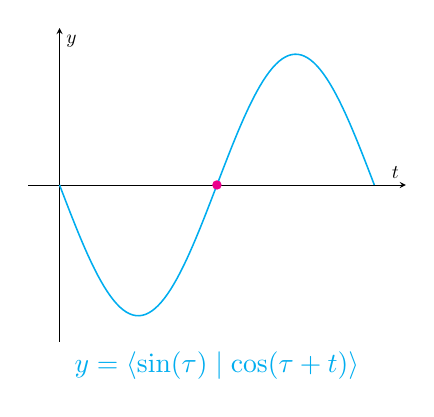
\begin{tikzpicture}[scale=0.7]
	\begin{axis}[axis lines=middle,
		            xlabel=$t$,
		            ylabel=$y$,
	           	 enlargelimits,
           		 ytick=\empty,
		            xtick=\empty
           	 ]
		
		\addplot[name path=F,cyan,thick,domain={0:6.28},samples=100] {-3.14*sin(x*180/3.14)};
		\addplot[magenta,thick,mark=*] coordinates{({4*0.785},{-3.14*sin((4*0.785)*180/3.14))})};
	\end{axis}
	\node[below,cyan] at (current bounding box.south) {$y=\braket{\sin(\tau)}{\cos(\tau+t)}$};
\end{tikzpicture}




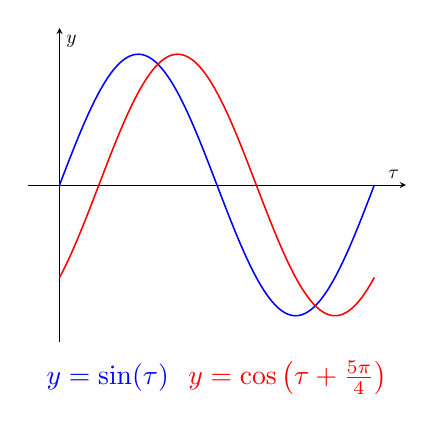
\begin{tikzpicture}[scale=0.7]
	\begin{axis}[axis lines=middle,
		            xlabel=$\tau$,
		            ylabel=$y$,
	           	 enlargelimits,
           		 ytick=\empty,
		            xtick=\empty
           	 ]
		
		\addplot[name path=F,blue,thick,domain={0:6.28},samples=100] {2*sin(x*180/3.14)};

		\addplot[name path=G,red,thick,domain={0:6.28},samples=100] {2*cos((x+5*0.785)*180/3.14)};
	\end{axis}
		\matrix[below] at (current bounding box.south){
			\node[blue,left] {$y=\sin(\tau)$};
			\node[red,right] {$y=\cos\left(\tau+\frac{5\pi}{4}\right)$};\\
		};
\end{tikzpicture}
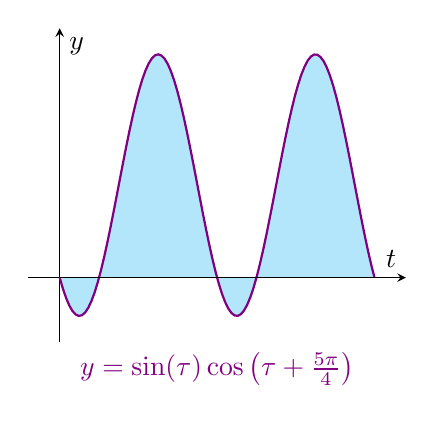
\begin{tikzpicture}[scale=0.7]
	\begin{axis}[axis lines=middle,
		            xlabel=$t$,
		            ylabel=$y$,
	           	 enlargelimits,
           		 ytick=\empty,
		            xtick=\empty
           	 ]
		
		\addplot[name path=F,violet,thick,domain={0:6.28},samples=100] {2*sin(x*180/3.14)*cos((x+5*0.785)*180/3.14)};

		\addplot[name path=G,domain=0:6.28] {0};

		\addplot[cyan!30] fill between [of=F and G];
	\end{axis}
	\node[below,violet] at (current bounding box.south) {$y=\sin(\tau)\cos\left(\tau+\frac{5\pi}{4}\right)$};
\end{tikzpicture}
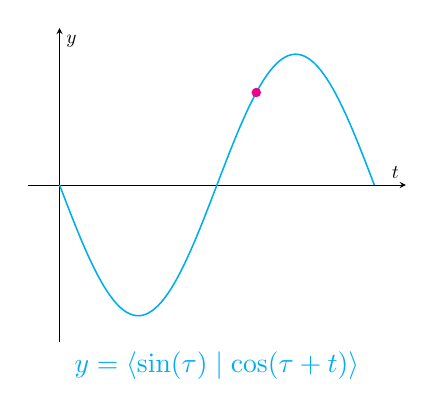
\begin{tikzpicture}[scale=0.7]
	\begin{axis}[axis lines=middle,
		            xlabel=$t$,
		            ylabel=$y$,
	           	 enlargelimits,
           		 ytick=\empty,
		            xtick=\empty
           	 ]
		
		\addplot[name path=F,cyan,thick,domain={0:6.28},samples=100] {-3.14*sin(x*180/3.14)};
		\addplot[magenta,thick,mark=*] coordinates{({5*0.785},{-3.14*sin((5*0.785)*180/3.14))})};
	\end{axis}
	\node[below,cyan] at (current bounding box.south) {$y=\braket{\sin(\tau)}{\cos(\tau+t)}$};
\end{tikzpicture}




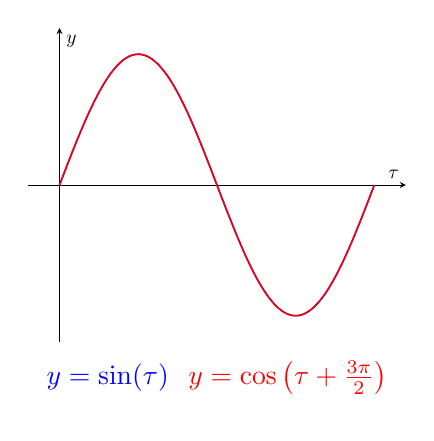
\begin{tikzpicture}[scale=0.7]
	\begin{axis}[axis lines=middle,
		            xlabel=$\tau$,
		            ylabel=$y$,
	           	 enlargelimits,
           		 ytick=\empty,
		            xtick=\empty
           	 ]
		
		\addplot[name path=F,blue,thick,domain={0:6.28},samples=100] {2*sin(x*180/3.14)};

		\addplot[name path=G,red,thick,domain={0:6.28},samples=100] {2*cos((x+6*0.785)*180/3.14)};
	\end{axis}
		\matrix[below] at (current bounding box.south){
			\node[blue,left] {$y=\sin(\tau)$};
			\node[red,right] {$y=\cos\left(\tau+\frac{3\pi}{2}\right)$};\\
		};
\end{tikzpicture}
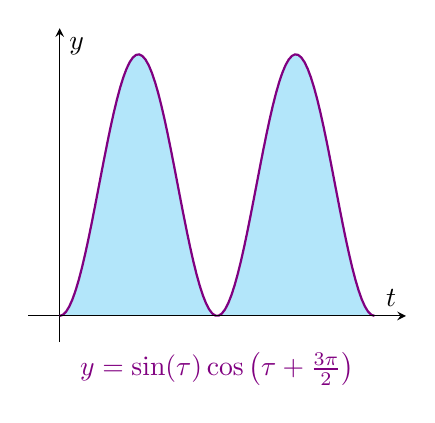
\begin{tikzpicture}[scale=0.7]
	\begin{axis}[axis lines=middle,
		            xlabel=$t$,
		            ylabel=$y$,
	           	 enlargelimits,
           		 ytick=\empty,
		            xtick=\empty
           	 ]
		
		\addplot[name path=F,violet,thick,domain={0:6.28},samples=100] {2*sin(x*180/3.14)*cos((x+6*0.785)*180/3.14)};

		\addplot[name path=G,domain=0:6.28] {0};

		\addplot[cyan!30] fill between [of=F and G];
	\end{axis}
	\node[below,violet] at (current bounding box.south) {$y=\sin(\tau)\cos\left(\tau+\frac{3\pi}{2}\right)$};
\end{tikzpicture}
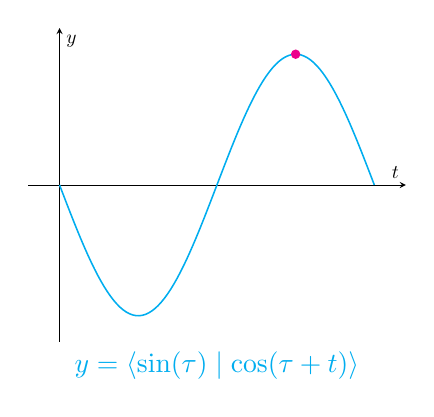
\begin{tikzpicture}[scale=0.7]
	\begin{axis}[axis lines=middle,
		            xlabel=$t$,
		            ylabel=$y$,
	           	 enlargelimits,
           		 ytick=\empty,
		            xtick=\empty
           	 ]
		
		\addplot[name path=F,cyan,thick,domain={0:6.28},samples=100] {-3.14*sin(x*180/3.14)};
		\addplot[magenta,thick,mark=*] coordinates{({6*0.785},{-3.14*sin((6*0.785)*180/3.14))})};
	\end{axis}
	\node[below,cyan] at (current bounding box.south) {$y=\braket{\sin(\tau)}{\cos(\tau+t)}$};
\end{tikzpicture}




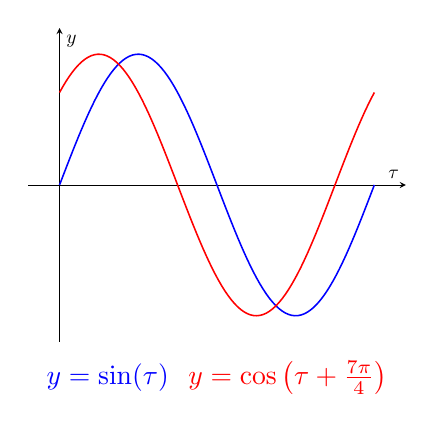
\begin{tikzpicture}[scale=0.7]
	\begin{axis}[axis lines=middle,
		            xlabel=$\tau$,
		            ylabel=$y$,
	           	 enlargelimits,
           		 ytick=\empty,
		            xtick=\empty
           	 ]
		
		\addplot[name path=F,blue,thick,domain={0:6.28},samples=100] {2*sin(x*180/3.14)};

		\addplot[name path=G,red,thick,domain={0:6.28},samples=100] {2*cos((x+7*0.785)*180/3.14)};
	\end{axis}
		\matrix[below] at (current bounding box.south){
			\node[blue,left] {$y=\sin(\tau)$};
			\node[red,right] {$y=\cos\left(\tau+\frac{7\pi}{4}\right)$};\\
		};
\end{tikzpicture}
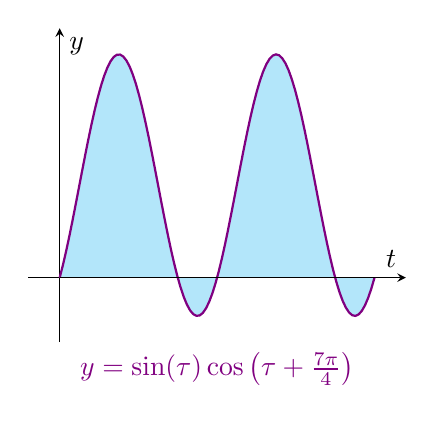
\begin{tikzpicture}[scale=0.7]
	\begin{axis}[axis lines=middle,
		            xlabel=$t$,
		            ylabel=$y$,
	           	 enlargelimits,
           		 ytick=\empty,
		            xtick=\empty
           	 ]
		
		\addplot[name path=F,violet,thick,domain={0:6.28},samples=100] {2*sin(x*180/3.14)*cos((x+7*0.785)*180/3.14)};

		\addplot[name path=G,domain=0:6.28] {0};

		\addplot[cyan!30] fill between [of=F and G];
	\end{axis}
	\node[below,violet] at (current bounding box.south) {$y=\sin(\tau)\cos\left(\tau+\frac{7\pi}{4}\right)$};
\end{tikzpicture}
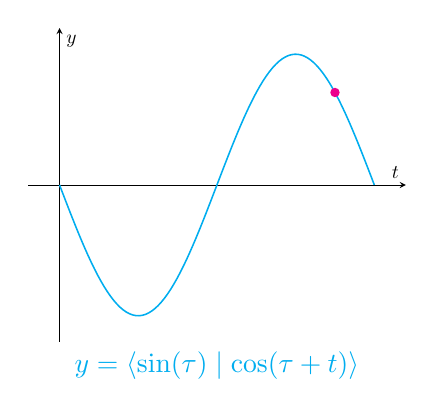
\begin{tikzpicture}[scale=0.7]
	\begin{axis}[axis lines=middle,
		            xlabel=$t$,
		            ylabel=$y$,
	           	 enlargelimits,
           		 ytick=\empty,
		            xtick=\empty
           	 ]
		
		\addplot[name path=F,cyan,thick,domain={0:6.28},samples=100] {-3.14*sin(x*180/3.14)};
		\addplot[magenta,thick,mark=*] coordinates{({7*0.785},{-3.14*sin((7*0.785)*180/3.14))})};
	\end{axis}
	\node[below,cyan] at (current bounding box.south) {$y=\braket{\sin(\tau)}{\cos(\tau+t)}$};
\end{tikzpicture}
\end{center}







\clearpage












\textbf{Theory: Convolution:}\bigskip


The cross-correlation of two functions $f$ and $g$ tells you, for each $t$, broadly how similar $f(\tau)$ and $g(\tau+t)$ are. There is a similar notion, called the \textbf{convolution} of $f$ and $g$, denoted $(f\ast g)(t)$, which tells you for each $t$ how similar $f(\tau)$ and $g(t-\tau)$ are; so the convolution of $f(t)$ with $g(t)$ is simply the cross-correlation of $f(t)$ with $g(-t)$.

Above, we considered the cross-correlation of periodic functions, sine and cosine, so it made sense to integrate over one period. In general, we will integrate over the whole positive real line. So
\[(f\ast g)(t)=\int_{0}^\infty f(\tau)g(t-\tau)\diff \tau.\]
Of course, this integral might not converge; if $f$ and $g$ are nice enough functions, it will. If the integral does not converge, then by broadening our notion of functions to include function\textit{als} like the Dirac delta, we can often still convolve $f$ and $g$, just as we can take Fourier transforms of functions that do not decay quickly enough toward $\infty$.\bigskip



Suppose we have two time-domain functions, $f(t)$ and $g(t)$, whose Laplace transforms $F(s)$ and $G(s)$ are known. Can we use this to compute the Laplace transform of the convolution, $f\ast g$? We have:
\begin{align*}
	\mathcal{L}\left({f\ast g}\right)(s) &=\int_{0}^\infty (f\ast g)(t)e^{-st}\diff t\\
	&=\int_{0}^\infty\int_{0}^\infty f(\tau)g(t-\tau)\diff \tau\,e^{-s t}\diff t\\
	&=\int_0^\infty\int_0^\infty f(\tau)g(t-\tau)e^{-s t}\diff \tau\diff t.
\end{align*}

Now we substitute $\sigma=t-\tau$ in the outer integral (so $\diff \sigma =\diff t$):
\begin{align*}
	\mathcal{L}\left({f\ast g}\right)(s)&= \int_0^\infty\int_0^\infty f(\tau)g(\sigma)e^{-s (\tau+\sigma)}\diff \tau\diff\sigma\\
	&=\int_0^\infty \int_0^\infty f(\tau)e^{-s \tau}g(\sigma)e^{-s \sigma}\diff \tau\diff \sigma\\
	&=\int_0^\infty g(\sigma) e^{-s \sigma}\int_{0}^\infty f(\tau)e^{-s \tau}\diff \tau \diff\sigma\\
	&=\int_{0}^\infty f(\tau)e^{-s \tau}\diff \tau \int_{0}^\infty g(\sigma)e^{-s \sigma}\diff\sigma\\
	&=F(s)G(s).
\end{align*}


\clearpage


\textbf{Theory: Convolution (cont.):}\bigskip


So for time-domain functions $f$ and $g$, the Laplace transform of the convolution is the product of the individual Laplace transforms:
\[\mathcal{L}(f\ast g) = \mathcal{L}(f)\mathcal{L}(g).\]
We usually express this by saying that convolution in the time domain corresponds to multiplication in the Laplace domain.

The converse is also true, with some slight caveats: multiplication in the time domain corresponds to convolution in the Laplace domain:
\[\mathcal{L}(fg)(s)=\frac{1}{2\pi j}\int_{-\infty}^\infty \mathcal{L}(f)(a+\sigma j) \mathcal{L}(g)(s-(a+\sigma j))\diff \sigma,\]
where $a$ is large enough that the domain of integration is entirely within the domains of convergence of $\mathcal{L}(f)$ and $\mathcal{L}(g)$. Comparing with Mellin's inverse formula, we see that this means
\[\mathcal{L}(fg)(s)=\mathcal{L}(f)(a+\sigma j)\ast\mathcal{L}(g)(a+\sigma j)\]
for large enough $a$.

The proof of the converse formula is essentially the same as the proof of the forward formula; simply apply the manipulations we did on the last page in Mellin's inverse formula.\bigskip


The direct use of this relationship between multiplication and convolution is that if we know the Laplace transforms of functions $f$ and $g$, and wish to find the transform of $fg$, it might be easier to convolve the transforms of $f$ and $g$ than to directly take the transform of $fg$.

Moreover, convolution itself has many applications; for instance, many filtering processes in electronics, acoustics, and optics, amount to convolving a signal with some noise or lens function. In probability, if $X$ and $Y$ are random variables, the probability distribution of $X+Y$ is found by convolving the distributions of $X$ and of $Y$. The Laplace transform allows us to convert convolution problems such as this into multiplication problems.\bigskip


Another use of the Convolution Theorem is that it allows us to prove properties of convolution by relating them to properties of multiplication. For instance, to prove that $f\ast g=g\ast f$, we could work from the definition by the integral, but it's easier just to take the Laplace transform, note that $\mathcal{L}(f)\mathcal{L}(g)=\mathcal{L}(g)\mathcal{L}(f)$, then take the inverse transform.






\clearpage



\textbf{Practice:}\bigskip

\begin{enumerate}
	\item Let $g(t)=\delta(t-\alpha)$. Show that for any function $f$,
		\[(f\ast g)(t)=f(t+\alpha).\]
		In particular, when $\alpha=0$, $f\ast \delta=f$, so convolving with the Dirac delta does not change a function.
	\item Recall from the last sheet that $\mathcal{L}(e^{\alpha t})=\frac{1}{s-\alpha}$ for any constant $\alpha$.
		\begin{enumerate}
			\item Show that
				\[\mathcal{L}(\sin(\omega t))=\frac{1}{2j}\left(\frac{1}{s-j\omega}-\frac{1}{s+j\omega}\right)=\frac{\omega}{s^2+\omega^2}.\]
			\item Hence show that
				\[\mathcal{L}\left(e^{\alpha t}\ast\sin(\omega t)\right) = \frac{\omega}{(s-\alpha)(s^2+\omega^2)}.\]
		\end{enumerate}
	\item Let $f$, $g$, and $h$ be functions. Show that
		\[(f\ast g)\ast h = f\ast(g\ast h).\]
\end{enumerate}















\clearpage




{\bf Key Points to Remember:}

\vspace{5mm}

\begin{enumerate}
	\item The \textbf{convolution} of two functions $f$ and $g$ is the function $f\ast g$ defined by
		\[(f\ast g)(t)=\int_{-\infty}^\infty f(\tau)g(t-\tau)\diff \tau.\]
		It gives a measure, for each $t$, of how much $f(\tau)$ and $g(-\tau)$ are similar (in terms of having the same sign) when $g(-\tau)$ is translated by $t$.
	\item The \textbf{convolution theorem} states that convolution and multiplication are dual under the Laplace transform:
		\begin{align*}
			\mathcal{L}(f\ast g) &= \mathcal{L}(f)\mathcal{L}(g)\\
			\mathcal{L}(fg)&=\mathcal{L}(f)\ast \mathcal{L}(g),
		\end{align*}
		where the convolution in the Laplace domain is taken with respect to the imaginary part, for a fixed real part large enough that both Laplace transforms converge.
	\item Convolution with a Dirac delta is translation:
		\[f(t)\ast \delta(t-\alpha) = f(t+\alpha)\]
		for any function $f$.
\end{enumerate}









\end{document}